\documentclass{standalone}
\usepackage{tikz}
\usepackage{hsbcommon}
    \begin{document}
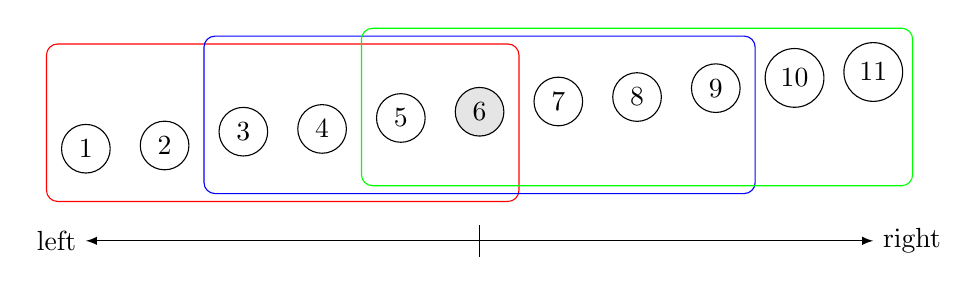
\begin{tikzpicture}
        \pgfmathsetseed{1}
        \draw[->,>=latex] (0,0) -- (-5,0) node[left] {left};
        \draw (0,0.2) -- (0,-0.2);
        \draw[->,>=latex] (0,0) -- (5,0) node[right] {right};;

        \foreach [count=\i] \ii in {-5,-4,...,5}
        {
            \pgfmathsetmacro\myy{rnd*(0.1)}
            \ifnum\ii=0
            \node[draw,fill=gray!20,circle] at (\ii,\i/10+\myy+1) {\i};
            \else
            \node[draw, circle] at (\ii,\i/10+\myy+1) {\i};
            \fi
        }
    

        \ifstep{1}{
\begin{scope}[color=red]

            \draw[rounded corners] (-5.5,0.5) rectangle (0.5,2.5);
        \end{scope}
}

        \ifstep{1}{
\begin{scope}[color=blue,yshift=0.1cm]

            \draw[rounded corners] (-3.5,0.5) rectangle (3.5,2.5);
        \end{scope}
}

        \ifstep{1}{
\begin{scope}[color=green,yshift=0.2cm]

            \draw[rounded corners] (-1.5,0.5) rectangle (5.5,2.5);
        \end{scope}
}

        
    \end{tikzpicture}
\end{document}
